\documentclass[12pt, a4paper]{report}
\edef\restoreparindent{\parindent=\the\parindent\relax}
\usepackage{fontspec}
\usepackage[UKenglish]{babel}
\usepackage[bibstyle=ieee, dashed=false, sorting=nty]{biblatex}
\usepackage[labelfont=bf]{caption}
\usepackage{colortbl}
\usepackage{csquotes}
\usepackage{fancyhdr}
\usepackage{float}
\usepackage{graphicx}
\usepackage[hidelinks]{hyperref}
\usepackage[toc, acronym, automake, nomain]{glossaries} % after hyperref for link
\usepackage{import}
\usepackage{listings}
\usepackage{longtable}
\usepackage{microtype}
\usepackage{multicol}
\usepackage{parskip}
\usepackage[dvipsnames]{xcolor}
\usepackage{pgfplots, tikz}
\usepackage{subcaption}
\usepackage[edges]{forest}

\linespread{1.2}
\restoreparindent

\lstset{captionpos=b, columns=flexible}

\pgfplotsset{small, compat=1.16}
\usepgfplotslibrary{dateplot}
\usetikzlibrary{fpu, positioning, shapes}

\definecolor{folderbg}{RGB}{124,166,198}
\definecolor{folderborder}{RGB}{110,144,169}
\newlength\Size
\setlength\Size{4pt}
\tikzset{%
  folder/.pic={%
    \filldraw [draw=folderborder, top color=folderbg!50, bottom color=folderbg]
    (-1.05*\Size,0.2\Size+5pt) rectangle ++(.75*\Size,-0.2\Size-5pt); \filldraw [draw=folderborder,
    top color=folderbg!50, bottom color=folderbg] (-1.15*\Size,-\Size) rectangle (1.15*\Size,\Size);
  },
  file/.pic={%
    \filldraw [draw=folderborder, top color=folderbg!5, bottom color=folderbg!10]
    (-\Size,.4*\Size+5pt) coordinate (a) |- (\Size,-1.2*\Size) coordinate (b) -- ++(0,1.6*\Size)
    coordinate (c) -- ++(-5pt,5pt) coordinate (d) -- cycle (d) |- (c) ;
  },
}
\forestset{%
  declare autowrapped toks={pic me}{},
  pic dir tree/.style={%
    for tree={folder, font=\ttfamily, grow'=0},
    before typesetting nodes={%
      for tree={edge label+/.option={pic me},},
    },
  },
  pic me set/.code n args=2{%
    \forestset{%
      #1/.style={inner xsep=2\Size, pic me={pic {#2}},}
    }
  },
  pic me set={directory}{folder},
  pic me set={file}{file},
}

\pagestyle{fancy}
\fancyhf{}
\fancyhead[C]{\leftmark}
\fancyfoot[C]{\thepage}

\makeglossaries
\renewcommand*{\glstextformat}[1]{\textbf{#1}}
\newacronym{apis}{APIs}{application processing interfaces}
\newacronym{cli}{CLI}{Command-line Interface}
\newacronym{cve}{CVE}{Common Vulnerabilities and Exposures}
\newacronym{cwe}{CWE}{Common Weakness Enumeration}
\newacronym{floss}{FLOSS}{Free/Libre and Open Source Software}
\newacronym{gui}{GUI}{Graphical User Interface}
\newacronym{hpc}{HPC}{High Performance Computing}
\newacronym{json}{JSON}{JavaScript Object Notation}
\newacronym{msr}{MSR}{Mining Software Repositories}
\newacronym{nvd}{NVD}{National Vulnerability Database}
\newacronym{oop}{OOP}{Object-oriented Programming}
\newacronym{owasp}{OWASP}{Open Web Application Security Project}
\newacronym{stdout}{stdout}{Standard Output}
\newacronym{xml}{XML}{Extensible Markup Language}

\addbibresource{references.bib}

\begin{document}
\begin{titlepage}
  \centering
  \includegraphics[width=10cm]{images/tuos_logo}\par\vspace{1cm}
  \vspace{1cm}

  {\huge\bfseries Finding Security Issues in (Open Source) Software Repositories\par}
  \vspace{1cm}

  {\Large Zer Jun Eng\par}
  \vspace{1cm}

  supervised by\par Dr.~Achim \textsc{Brucker}
  \vfill

  {This report is submitted in partial fulfilment of the requirement for the degree of MEng Software
    Enginnering by Zer Jun Eng}
  \vfill

  {\large COM3610}
  \vfill

  {\large \today}
\end{titlepage}

\pagenumbering{roman}

\chapter*{Declaration}
All sentences or passages quoted in this report from other people's work have been specifically
acknowledged by clear cross-referencing to author, work and page(s). Any illustrations that are not
the work of the author of this report have been used with the explicit permission of the originator
and are specifically acknowledged. I understand that failure to do this amounts to plagiarism and
will be considered grounds for failure in this project and the degree examination as a whole.
\vspace{2cm}

\noindent \begin{tabular}{llp{4.5cm}}
  Name & : & Zer Jun Eng \\ \cline{3-3}
  \\ [-0.5em]
  Date & : & \today      \\ \cline{3-3}
\end{tabular}

\newpage

\chapter*{Abstract}
% In both proprietary and Free/Libre and Open Source Softwares (FLOSS) components, not all security
% vulnerabilities are documented in CVE format nor published in the vulnerability databases such as
% NVD. These vulnerabilities could have been fixed by the developers. Finding these
% vulnerability-fixing commits could provide valuable insights for the developers using those
% components. Therefore, the objective of this project is to develop a repository mining tool that
% is able to detect vulnerability-fixing commits using MSR approach. Comparing to previous
% approaches, the tool will be focusing on searches the commit message first, and then investigates
% the code difference in each commit.

\chapter*{Acknowledgements}
I would like to thank my parents for their unconditional love and the full financial support
throughout my university life. It would not be possible for me to finish this project and my course
without them.

I would also like to thank my supervisor, Dr. Achim Brucker for continuously providing constructive
advice for my project. I am honoured to work with you, and I look forward to working with you in the
future.

\newpage

\tableofcontents

\listoffigures

\listoftables

\lstlistoflistings

\newpage

\pagenumbering{arabic}

\chapter{Introduction}
\section{Background}
\acrfull{floss} is a type of software whose license allows the users to inspect, use, change and
redistribute the software's source code \cite{crowston_2012}. Since the introduction of the version
control system, many repository hosting sites such as SourceForge \cite{sourceforge}, Google Code
\cite{google_code}, and GitHub \cite{github} have been launched. As a result, the participation of
global communities into \acrshort{floss} projects have started to grow and different contributions
were made to improve the software quality, which included fixing software vulnerabilities
\cite{dabbish_2012}.

Building secure software is expensive, difficult, and time-consuming. It is necessary to know when
and how a security vulnerability is fixed throughout the software lifecycle. Software components
such as plugins and \acrfull{apis} are usually developed by third-party developers and widely reused
in both open source and closed source software \cite{khan_2001}. An important factor of software
security is determined by the information provided by the vendor of the software components for
deciding whether to perform the security update. Hence, the users of software components are advised
to check the \acrfull{nvd} \cite{nvd} regularly for detailed information of the vulnerabilities
identified in the software components used. Furthermore, it would be more helpful if the developers
of the software components recorded the list of changes or provide informative Git commit messages
for every version update of their component.

To perform a risk assessment of a potentially vulnerable component, it is required to have a deep
understanding of the vulnerability entry points. Yet, not all projects follow the \acrfull{cve}
format or publish \acrshort{cve}, and \acrshort{cve} reports are usually lack of technical details
that attribute the specific entry points of the vulnerability, which is an important aspect in part
of the risk assessment. By identifying the vulnerability-fixing commits, the vulnerable lines of
code can be located, which allows the users to check if a vulnerable component is being used or not.
However, some developers believe that public disclosure of security vulnerabilities patch is
dangerous, thus vulnerability-fixing commits are not commonly identified and recorded specifically
in some open source software repositories to prevent malicious exploits \cite{arora_2005}. As a
result, there is a practical difficulty in applying this analysis approach to find the security
relevant commits that are not documented using \acrshort{cve} or a similar format, which are known
as the silent patches.

To address these issues, a repository mining tool that investigates commit messages and identifies
vulnerable software components can be developed to reduce the time and cost required to mitigate the
vulnerabilities. The repository mining tool should be able to detect the silent patches through an
advanced process, which the tool must analyse the source code changes between commits to locate the
vulnerable lines of code. Moreover, the mining tool should be applicable to all types of software
projects that are using Git as their version control system. Projects that are using a different
version control system are also supported after they have been migrated to Git.

\section{Objectives} \label{sec:objectives}
\begin{itemize}
  \item Identify the security patterns of the security issues in the \acrfull{owasp}
  Top Ten Project. The tool is aimed to cover the most common or important security issues in the
  list.
  \item Develop a repository mining tool to search through the commit history of a repository and
  find a list of commit messages that match the patterns. The list should be produced in
  \acrfull{json} file format.
  \item Extend the mining tool which checks the code difference in the commits found to obtain the
  actual commits fixing the security vulnerabilities.
  \item Create a statistical tool that reads the output file and reports a detailed analysis of the
  results.
\end{itemize}

\section{Challenges} \label{sec:challenges}
This section is a brief summary of the main challenges that might occurred during the project. A
more thorough analysis of the problems and constraints is carried out in
\hyperref[sec:problems_and_constraints]{\textbf{Section \ref*{sec:problems_and_constraints}}}.

\begin{itemize}
  \item \textbf{Data:} There are a large number of open source repositories available on GitHub.
  However, it is challenging to find a set of sample repositories that can produce accurate and
  consistent results.
  \item \textbf{Misclassification:} The commit messages for the same vulnerability patch are not
  always the same, thus misclassification is inevitable. Using regular expressions to match the
  patterns in the mining process do not guarantee the correctness of the result.
  \item \textbf{Evaluation:} After mining a list of commits that contain the identified patterns in
  its message, the evaluation process might not correctly locate the lines of code that addressed
  the security vulnerability. It might be required to perform a manual evaluation to correctly
  identify some of the results.
  \item \textbf{Time:} Large repository such as Linux which has more than 820,000 commits in total
  \cite{linux_repo} could be extremely time-consuming for the repository mining tool to complete the
  search and evaluation process.
\end{itemize}

\section{Report Structure}
\textbf{Chapter 2} reviews a range of academic articles, theories, and previous studies that is
related to this project, as well as investigating the techniques and tools to be used.

\noindent\textbf{Chapter 3} is a list of detailed requirements and a thorough analysis of design,
implementation and testing stage. Some core decisions are reviewed in the analysis part to ensure
the feasibility of the project.

\noindent\textbf{Chapter 4} is a comparison between different design concepts, where the advantages
and disadvantages of different approaches are stated. The chosen design is justified with suitable
diagrams provided including wireframes and UML component diagrams.

\noindent\textbf{Chapter 5} describes the implementation process by highlighting novel aspects to
the algorithms used. Testing is performed by following a suitable model to evaluate the
implementation.

\noindent\textbf{Chapter 6} presents all the results along with critical discussions about the main
findings,	and outlines the possible improvements that could be made in the future work.

\noindent\textbf{Chapter 7} summarises the main points of previous chapters and emphasise the
results found.

\section{Relationship to Degree Programme}
This project focuses on the research of real-world software security problems and offers valuable
insights into computer security. By studying the patterns of security vulnerabilities patch in open
source repositories, the practical knowledge for building and ensuring a secure system could be
gained. Moreover, the difficulty of improving software security could be experienced during the
evaluation process in this project. This relates to the Software Engineering degree as it requires a
good understanding in version control system and it aims to improve softwares quality by reducing
the time and effort needed to find security vulnerabilities in the source code.

\chapter{Literature Review}
This chapter will start with the background contents of the project, and then focus on discussing
the security aspect of open source softwares. Additionally, previous and existing relevant works are
reviewed and a critical analysis is provided for the comparison of these resources and this project.

\section{Open Source Security}
The security of open source softwares mostly rely on the collaboration of the community. It is
deduced that the power of open data and crowdsourcing will make open source security more reliable
\cite{hoepman_2007, witten_2001}, and provides more flexibility and freedom over the security option
to their users \cite{payne_2002}. However, when it comes to publishing the vulnerability
information, it is suggested that the list of unconfirmed vulnerabilities should not be published
publicly to protect the users from potential harms \cite{schryen_2011}.

Arora, Nandkumar and Telang \cite{arora_2006} have shown that vulnerabilities that are either secret
or published but not patched attract fewer attacks than patched vulnerabilities. Although the
research was conducted in 2006 and the results might be outdated, it still implies that developers
might include a silent patch into some of the commits that is not explicitly recorded in the commit
messages. It might be a rational approach for not disclosing the work attempted to fix a
vulnerability, but other developers might not be informed of the content change. Furthermore, if a
similar vulnerability is discovered in the future, developers would need more effort for finding the
previous solution. Therefore, it would be very useful for the developers if the mining tool
developed in this project could detect the silent patches.

\section{Taxonomy of Software Vulnerabilities}
There are many software vulnerabilities being identified each year. By using a common vulnerability
identifier system, vulnerability data can be shared across separate vulnerability databases to
facilitate the interoperability of different tools. As this project focuses on finding security
issues in open source repositories, it is necessary to discuss the industry-endorsed standard of
software vulnerabilities categorisation.

\subsection{Common Weakness Enumeration}
The \acrfull{cwe} is a project launched by the Mitre Corporation and sponsored by the National Cyber
Security Division of the United States Department of Homeland Security \cite{cwe}. The
\acrshort{cwe} project organises the software weaknesses into a list of different categories, known
as the \acrshort{cwe} list. Software weaknesses are defined as errors that can lead to software
vulnerabilities, which includes buffer overflows, authentication errors, code injection, etc.
\cite{cwe_faq}. The \acrshort{cwe} is now a formal standard for representing software weaknesses.
Each entry in the \acrshort{cwe} list contains detailed information about the specific weakness and
is identified by a unique ID number.

\subsection{Common Vulnerabilities and Exposures}
The \acrfull{cve} is another security project launched by the Mitre Corporation \cite{cve} to
provide the community with a complete list of publicly known security vulnerabilities, known as the
\acrshort{cve} entries. Each \acrshort{cve} entry is defined by an ID number, and includes a
description followed by any relevant resources about the vulnerability. It is now the standardised
solution and industry-recognised standard for identifying vulnerabilities and exposures. However,
developers and vendors are not required to publish security vulnerabilities of their projects
\acrshort{cve} format. They are allowed to use their own naming scheme for the vulnerabilities, even
if the same vulnerability has already been recorded in the \acrshort{cve} list.

\section{Security Issues in Open Source Softwares}
The \acrfull{owasp} is a worldwide non-profit organization committed to improve and raise the
awareness of software security \cite{owasp_home}. The project members of \acrshort{owasp} have
worked together to produce a list of the most critical web application security risks based on the
community feedback and comprehensive data contributed by different organizations. The list consists
of ten categories of security attacks which are considered to be the most dangerous and popular in
recent years. In \acrshort{owasp} Top Ten 2017 \cite{owasp_top10}, one of the vulnerabilities that
is closely related to this project is \hyperref[subsec:components]{`Using Components with Known
Vulnerabilities'}, which will be extensively discussed.

\subsection{Using Components with Known Vulnerabilities} \label{subsec:components}
It has been indicated that a small software component could create a large error in a software
system \cite{basili_1984, munson_1992, selby_1988}. Components such as plugins, libraries, and
modules are ubiquitous in both open source and proprietary softwares. Third-party components are
increasingly being integrated into softwares to reduce the amount of time and effort required for
development \cite{balzarotti_2006}, but they also increase the risk of vulnerabilities being
introduced into the softwares. These components are mostly maintained by different developers or
organisations, and the time required to fix a vulnerability varies between developers. While the
majority of third-party components are still being actively maintained after a long time, some of
them might have depreciated and security patches are no longer being released. The users might
continue to use a depreciated component if they could not find a better alternative. However, using
outdated components greatly increase the risk of software exploits. Therefore, for any large-scale
system, the developers must scan for vulnerabilities regularly and subscribe to the security news
related to the components used to reduce the risk of security vulnerabilities being introduced into
the system.

Vulnerable components can be found using methods ranging from dependency checking to machine
learning. While this project is related to the former approach, the latter approach concentrates on
finding the relationship between software errors and vulnerabilities to identify or predict
high-risk components. Dependency checking is an approach of detecting dependencies (plugins,
libraries, etc.) with known vulnerabilities in a software. Several open source tools including
\acrshort{owasp} Dependency Check \cite{owasp_dependency}, Retire.js \cite{retirejs}, and Safety
\cite{safety} are applications that identifies vulnerable dependencies in a software project.
Cadariu et al. \cite{cadariu_2015} have used the \acrshort{owasp} Dependency Check tool to find all
known vulnerabilities that have a unique \acrshort{cve} identifier in proprietary softwares written
in Java. According to their study, the \acrshort{owasp} Dependency Check tool has low precision due
to the high false positives rate in the large data sets. However, Cadariu et al. \cite{cadariu_2015}
justified that the tool is still usable by taking into account that the checking process is
automated and any security issue found is considered a valuable information for the users.

Machine learning-based approaches are also applicable to find vulnerable components in a software
system. Briand, Basili and Hetmanski \cite{briand_1993} have developed a model with Optimised Set
Reduction (OSR) algorithm that uses set theory, predicate logic, probability, and vector in the
calculation. The model focused on identifying the components that are more likely to produce a large
number of errors and it was proved to be effective, but the main drawbacks are the complexity of the
implementation and the extensive calculations required. In comparison to Briand's approach,
Scandariato et al. \cite{scandariato_2014} have built a model that uses text mining techniques to
predict vulnerable components. While Briand's model is capable of identifying high-risk components,
Scandariato's model is able to predict vulnerabilities in the future releases of a software
components, and the results achieved are satisfactory.

As a conclusion, static dependency checking tools provide a fast and easy way to scan for vulnerable
components, but the users are required to verify the validity and compatibility of the results with
their softwares. In contrast, models that use machine learning technique has been proved to be
effective and are more likely to produce consistent and accurate results. However, such models
require a large amount of training data and are only designed for a specific area. While dependency
checking approach is more related to the scope of this project, the capability of predicting
vulnerable software components through machine learning is a great way of preventing severe software
errors. In future work, machine learning could be incorporated into the tool developed in this
project to improve its overall effectiveness.

\section{Mining Software Repositories} \label{sec:msr}
\acrfull{msr} is a process of collecting and analysing data from repositories, which includes
version control repositories, mailing list repositories, and bug tracking repositories.
\acrshort{msr} applies to a wide range of fields such as business, research, and security
\cite{poncin_2011}. The purpose of \acrshort{msr} is to extract practical information from rich
metadata and discover hidden trends about a specific evolutionary characteristic \cite{kagdi_2007}.
The information collected could be used in various development process. For example, some developers
could gain insight by mining repositories, which may help them to enhance their software quality
based on previous implementation evidence of other developers \cite{hassan_2008}. While
\acrshort{msr} have various usages in different areas, the primary objective of this project will be
focusing on finding the security issues in open source software repositories through \acrshort{msr}.

In order to identify both hidden and publicly disclosed patches, it is required to make effective
use of \acrshort{msr} technique. A \acrshort{msr} process is normally carried out using tools or
scripts made by the researchers themselves. Although there are many types of research in the
\acrshort{msr} field in recent years, the majority of the tools or scrips used are not published
publicly \cite{robles_2010}. As a result, it is not possible to fully replicate the previous
research methods and make improvements based on that. Despite the undisclosed information of
research methods in many papers, Shang \cite{shang_2009} suggested that the \acrshort{msr} process
should be split into several stages, with each stage focusing on a specific topic of the problem to
achieve the optimal efficiency.

\subsection{Keywords Search}
For many complex approaches, the keywords searching process is considered to be the fundamental
step. If the initial results produced in the searching stage is good, a huge amount of effort could
be reduced in the later stages. However, the prerequisite is that the repository must have a
sufficient amount of valuable information, which can be estimated by judging the history of the
repository. To correctly and precisely retrieve the information for a query, it is required to
integrate some algorithms and modules into the search function. Matsushita, Sasaki, and Inoue
\cite{matsushita_2005} developed a repository search system that makes use of two functions: lexical
analysis function and token comparing function. The system produced very detailed results by
deploying recursive search strategy using the keywords found into every commit. On the contrary,
Mockus and Votta \cite{mockus_2000} designed an automated program that makes use of normalisation,
word frequency analysis, and keyword clustering techniques to search the commit messages. Although
the program is able to retrieve the results that include the keywords, the algorithm is unable to
identify similar terms or inconsistent form of wording for the commit messages.

\subsection{Properties of Vulnerability-Fixing Commits}
For every vulnerability identified in a repository, the vulnerability-fixing process that involves
analysis, implementation, testing, and release will be executed \cite{othmane_2015}. Most of the
vulnerability-fixing commits are pushed during the implementation and testing stage of the process.
However, if the commit message of a fixing commit is ambiguous, it will be challenging for any tools
to determine the correctness of the commit. In order to analyse the common features of the
vulnerability-fixing commits, it is needed to find these commits in open source repositories first.
By analysing the properties of vulnerability-fixing commits, it will ease the implementation of the
repository mining tool and enhance the quality of the regular expressions used.

Meneely et al. \cite{meneely_2013} conducted a research to study the properties of commits that
introduce vulnerabilities, in which a reverse approach was used to find vulnerability-contributing
commit by backtracking from the vulnerability-fixing commits. Meneely et al. identified the
vulnerability-fixing commits by investigating into each vulnerability manually to find the
respective fixing commit. However, the process of identifying vulnerability-fixing commit was not
clearly explained by them, thus no constructive information about the properties of
vulnerability-fixing commits is provided. On the contrary, V{\'a}squez, Bavota and Vel{\'a}squez
\cite{linares_2017} discovered that some vulnerability-fixing commits are grouped with other commits
to address a vulnerability, which matches the assumption of Neuhaus and Plattner
\cite{neuhaus_2013}, and thus only part of the code commited is related to the vulnerability fix.

\begin{figure}[H]
  \centering
  \begin{subfigure}{\textwidth}
    \centering
    \includegraphics[width=.7\textwidth]{images/vuln_fixing_commit_good_ex.png}
    \subcaption{Vulnerability fix in Linux kernel repository \cite{good_vfc}}
    \label{figure:g_vfc}
  \end{subfigure} \\
\end{figure}
\begin{figure}[H]\ContinuedFloat
  \begin{subfigure}{\textwidth}
    \centering
    \includegraphics[width=.7\textwidth]{images/vuln_fixing_commit_bad_ex.png}
    \subcaption{Vulerability fix in oauth2 proxy repository \cite{bad_vfc}}
    \label{figure:bad_vfc}
  \end{subfigure}
  \caption[Examples of vulnerability-fixing commit.]%
  %
  {A comparison of \hyperref[figure:g_vfc]{\textbf{(a)}} a higher quality and
    \hyperref[figure:bad_vfc]{\textbf{(b)}} a lower quality vulnerability-fixing
    commit.}
  \label{figure:comparion_vfc}
\end{figure}

\subsection{Finding Security Vulnerabilities} \label{subsec:finding_vuln}
It has been reported that the descriptions and references in vulnerability databases are often lack
of complete documentation \cite{massacci_2010}, and vulnerability-fixing commit are not ubiquitous
in every open source repository \cite{walden_2014}. Finding a security vulnerability could be hard
if the resources available are limited. Having completed the researches on keywords searching
techniques and properties of vulnerability-fixing commit, the approach for finding vulnerabilities
can now be reviewed.

In this project, a static repository mining tool will be developed to find security vulnerabilities
in open source repositories. Previous researches included the use of static software auditing and
vulnerability mitigation tools to find bugs and vulnerabilities \cite{cowan_2003}. However, Bessey
et al. \cite{bessey_2010} claimed that static tools have a negative effect on technical development
due to its high false positives rate. While this statement might be true, it does not imply that all
static tools are not effective as they differ in the techniques used in finding vulnerabilities
\cite{moser_2008}. Static tools usually require many experiments with different configurations to
obtain the best result, and the result may vary across different data sets. This project differs
from previous researches by aiming to find the security vulnerabilities through Git commit messages
first, and then analyse the code changes in the commits. Researches have shown that
vulnerability-fixing commits could be retrieved by extracting commit hashes from \acrshort{cve}
references and gathering all commits that refer to a \acrshort{cve} number in its commit message
\cite{jimenez_2016}, or by performing syntactic and semantic analysis on the commit messages
\cite{sliwerski_2005}. To verify the validity of the commits retrieved, a screening test
\cite{dashevskyi_2018} can be performed to investigate the code changes in a commit against several
criteria and identify the correct vulnerability-fixing commits.

This project extends prior work on Reis and Abreu's Secbench Mining Tool \cite{secbench}. The tool
aims to find vulnerabilities patch in GitHub repositories by using specific regular expressions for
each vulnerability pattern. Then it creates a test case for every vulnerability found and these test
cases are evaluated manually. Reis and Abreu \cite{reis_2017} discussed the procedure of the
evaluation and explained that human errors could occur due to source code complexity and similarity
of vulnerability pattern. The approach of Secbench Mining Tool is similar to the concept of this
project. However, performing manual evaluation on every result is not practical and it is proven
that the use of automated algorithms can improve the detection process \cite{livshits_2005}. In this
project, the tool developed should be able to automate the evaluation process to some extent, while
preserving the accuracy of the results.

\subsection{Source Code Analysis}
This section is an extension to \hyperref[subsec:finding_vuln]{\textbf{Section
\ref*{subsec:finding_vuln}}}. As this project involves in analysing the code changes in Git commits
using static analysis methods, it is necessary to review the techniques used to identify
vulnerabilities by source code analysis tools.

Finding vulnerabilities by source code analysis technique is relatively difficult than analysing
commit messages as it requires a high-level understanding in both software vulnerabilities and the
programming language of the source code. Source code analysis tools are generally designed for a
specific task, and only support specific programming languages \cite{antunes_2009}. There are two
types of analysis methods: static and dynamic. This project will mainly focus on studying static
analysis, and comparing its advantages and disadvantages with dynamic analysis.

One of the advantages of static source code analysis tool is that it can analyse the code without
executing it \cite{livshits_finding_2005}, but this could also be the drawback as it might generate
more false positives than dynamic analysis. Static analysis is considered to be a promising method
for detecting possible and obvious security vulnerabilities \cite{evans_2002}. Zitser, Lippmann, and
Leek \cite{zitser_2004} have developed a static code analysis tool to find buffer overflow
vulnerability in C programming language code. Their approach requires manual definitions of the
overflow patterns in their tool, which is considered to be a general method in static analysis.

\section{Improving Software Security with Static Analysis and Repository Mining}
The methods discussed in \hyperref[sec:msr]{\textbf{Section \ref*{sec:msr}}} could be used in
conjunction with static analysis tool to improve software security. As common static source code
analysis tools can only take one version of source code as input, it is unable to find security
vulnerabilities in previous version of the source code unless it is specifically provided to the
tool. Therefore, static analysis of source code could be integrated with \acrshort{msr} to find
potential security vulnerabilities in older versions of the source code.

Researches have suggested that users often turn off auto-updates for softwares \cite{fagan_2015,
mathur_2017} to avoid possible consequences such as major interface changes or compatibility issues.
This statement is justifiable if and only if an update does not introduce security improvements bug
fixes. As a result, it is helpful to run static analysis in an older version of software and inform
the users about the potential security vulnerabilities if the users decided not to update the
software. This can be done by traversing through the history of a given software repository and
reports the issues found in each revision, the implementation details are further explained in
\hyperref[chap:implementation]{\textbf{Chapter \ref*{chap:implementation}}}.

\section{Usage of the Repository Mining Tool in Other Areas}
While the repository mining tool developed in this project is only capable of finding security
issues through Git commits, it can be extended or modified to aid the researches in other areas.
Some examples are briefly discussed in the subsections below.

\subsection{Bugs Finding Model}
Both Williams and Hollingsworth \cite{williams_2005} and Ostrand and Weyuker \cite{ostrand_2004}
utilised \acrshort{msr} technique in their bugs finding model. Williams and Hollingsworth mined the
code changes in each commit to find possible bugs, while Ostrand and Weyuker mined the most
frequently modified files between version releases to predict the bugs-prone files.

\subsection{Machine Learning Model for Automated Vulnerability Prediction}
In comparison to the static approach used in the mining tool, machine learning technique could be
introduced to achieve higher reliability and accuracy on the result. Nguyen and Tran
\cite{nguyen_2010} and Perl et al. \cite{perl_2015} have built their machine learning model with
dependency graph and vulnerability-contributing commit as their main approach respectively, while Li
et al. \cite{li_2016} and Russell et al. \cite{russell_2018} used source code analysis method in
their machine learning model. According to their researches, machine learning models are able to
produce relatively high accuracy results.

\chapter{Requirements and Analysis}
The purpose of this chapter is to express the aims in details and discuss the problems to be solved.
This chapter will outline the requirements of the project and list the criteria to be met. The
analysis part will cover every aspect of the design, implementation, and testing stage to ensure
that the project is feasible.

\section{Project Objectives}
Initially, the objectives set in \hyperref[sec:objectives]{\textbf{Section \ref*{sec:objectives}}}
are an ideal concept of this project. Having completed the background research and literature
review, it is now possible to provide a detailed description and more clearly defined objectives
that improve the feasibility of this project.

\begin{enumerate}
  \item \textbf{Vulnerability patterns:} The term `vulnerability pattern' is used to represent the
  commit message pattern of different vulnerabilities. Correctly identifying the regular expression
  of each vulnerability pattern is time-consuming, and it would also need considerable refinement
  throughout the whole project. Hence, it might be more appropriate to reuse and improve the
  patterns provided in previous related works.
  \item \textbf{Mining the commits:} This task involves creating a repository mining tool that makes
  extensive use of the pre-defined regular expressions to search for the relevant commits. It is
  necessary to consider how closely a commit needs to match with the patterns for it to be included
  in the result. The file format for storing the results is \acrshort{json}, and reasons are
  justified in \hyperref[subsec:file_format]{\textbf{Section \ref*{subsec:file_format}}}.
  \item \textbf{Evaluating the mined commits:} The mining tool can be extended to include a separate
  function that evaluates the commits mined to find the actual code commit addressing the security
  vulnerabilities. This project will consider to automate the evaluation process to some extent
  while maintaining the accuracy of the results at the standard level.
\end{enumerate}

\section{Software Requirements and Scope} \label{sec:software_req}
\subsection{Functional Requirements}
\begin{longtable}{|p{10.3cm}|c|}
  \hline \endfirsthead
  \rowcolor[HTML]{D8D8D8}
  \multicolumn{1}{|c|}{Criteria} & Importance \\ \hline
  \textbf{Compatibility:} The mining tool should be able to run on all machines that meet the
  system requirements. & Essential \\ \hline
  \textbf{Completeness:} The mining tool should be able to find all relevant commits of security
  vulnerabilities based on the regular expressions. & Essential \\ \hline
  \textbf{Informative:} The statistical tool should return a complete analysis of the results. &
  Essential \\ \hline
  \textbf{Repeatable:} The results should be repeatable and reproducible. & Essential \\ \hline
  \textbf{Scalability:} The mining tool should be able to work on different project sizes, provided
  that the repository contains a certain amount of information. & Essential \\ \hline
  \textbf{Automated Evaluation:} The process of classifying and evaluating the commits into
  different vulnerabilities patch should be automated to a certain extent. & Desirable \\ \hline
  \textbf{Extensibility:} New vulnerability patterns and programming languages should be easily
  added into the tool. & Desirable \\ \hline
  \textbf{Robustness:} The mining tool should be able to handle all possible errors without
  terminating the mining process. & Desirable \\ \hline
  \caption{Functional requirements of the mining tool.} \label{table:func_req}
\end{longtable}

\subsection{Non-functional Requirements}
\begin{table}[H]
  \centering
  \begin{tabular}{|p{10.3cm}|c|}
    \hline
    \rowcolor[HTML]{D8D8D8}
    \multicolumn{1}{|c|}{Criteria} & Importance \\ \hline
    \textbf{Code Style:} The source code should be well-commented and follow a consistent coding
    style. & Essential  \\ \hline
    \textbf{Documentation:} Installation and user manual should be provided. & Essential \\ \hline
    \textbf{Lightweight:} The mining tool should have minimal dependencies. & Essential \\ \hline
    \textbf{Open source:} As the mining tool is built for researching open source repositories, it
    should be open source to suit the use cases. & Essential \\ \hline
    \textbf{Performance:} The performance of the mining tool should be optmised for different
    project sizes. & Desirable \\ \hline
  \end{tabular}
  \caption{Non-functional requirements of the mining tool.} \label{table:nonfunc_req}
\end{table}

\subsection{Scope}
In addition to \hyperref[table:func_req]{\textbf{Table \ref*{table:func_req}}} and
\hyperref[table:nonfunc_req]{\textbf{Table \ref*{table:nonfunc_req}}}, several fundamental
requirements can be included to define the scope of the mining tool.

\begin{itemize}
  \item \textbf{Language in Commit Messages:} The mining tool will only search for commit messages
  that are written in English.
  \item \textbf{Programming Language:} The source code analysis function in the mining tool will
  support C, C++, Python 3, and Java.
  \item \textbf{Repository type:} The mining tool will only support Git repositories. Hence,
  repositories using other version control systems such will have to convert to Git first before
  using the mining tool.
  \item \textbf{Vulnerability type:} It is aimed that the mining tool should be able to detect
  \acrshort{cve}-identified vulnerabilities that have been fixed and recorded in the commit message
  \hyperref[figure:cve_vuln]{\textbf{Figure \ref*{figure:fig_scope} (a)}}, and vulnerabilities that
  are not identified in \acrshort{cve} but recorded in the commit messages
  \hyperref[figure:common_vuln]{\textbf{Figure \ref*{figure:fig_scope} (b)}}.
\end{itemize}

\begin{figure}[H]
  \centering
  \begin{subfigure}{.5\textwidth}
    \centering
    \includegraphics[width=.85\textwidth]{images/cve_vuln.png}
    \subcaption{\acrshort{cve}-identified vulnerability fix \cite{cve_vuln}}
    \label{figure:cve_vuln}
  \end{subfigure}%
  \begin{subfigure}{.5\textwidth}
    \centering
    \includegraphics[width=.85\textwidth]{images/common_vuln.png}
    \subcaption{Common vulnerability fix \cite{common_vuln}}
    \label{figure:common_vuln}
  \end{subfigure}
  \caption[A comparison between a \acrshort{cve}-identified fixing commit and a common
  vulnerability-fixing commit.]%
  %
  {An example of \hyperref[figure:cve_vuln]{\textbf{(a)}} a \acrshort{cve}-identified vulnerability
    fix and \hyperref[figure:common_vuln]{\textbf{(b)}} a common vulnerability fix.}
  \label{figure:fig_scope}
\end{figure}

\section{Analysis}
The aim of this section is to contemplate the options available for this project and review some of
the fundamental decisions to be made before the implementation.

\subsection{Programming Language} \label{subsec:prog_lang}
Python 3 \cite{python} is chosen to be the main programming language for the repository mining tool.
While other programming languages may be more suitable for tackling specific problems of this
project, Python 3 provides sufficient coverage over every aspect with its comprehensive
functionality. The greatest advantage of Python 3 is that it has a wide range of libraries that
facilitate the development environment, which fully justified that a complete working solution can
be produced using Python 3.

\subsection{Libraries and Tools}
The Python 3 standard library contains a wide range of built-in modules and extensive facilities.
Moreover, many community created created tools can be integrated into Python programs with minimal
configurations as well. Below is a list of libraries and tools that will be used in the mining tool:
\begin{itemize}
  \item The \texttt{re} \cite{python_re} library for regular expression operations.
  \item The \texttt{json} \cite{python_json} library for creating and reading the result file.
  \item GitPython \cite{gitpython} is a Python library built to simplify the interaction with Git
  repositories.
  \item PyDriller \cite{pydriller_repo, spadini_2018} is a Python library built on top of GitPython
  with additional features for repository mining.
  \item Flawfinder \cite{flawfinder} is a program written in Python that is designed to find
  potential security vulnerabilities in C/C++ source code.
  \item Bandit \cite{bandit} is a tool created by the Python Code Quality Authority to find security
  issues in Python source code.
  \item graudit \cite{graudit} is a simple source code auditing tool that finds potential security
  vulnerabilities in source code using regular expression searches.
\end{itemize}

\subsection{File Format of Result} \label{subsec:file_format}
The \acrfull{json} \cite{json} has been chosen as the file format for storing the results in this
project. This is because \acrshort{json} is supported in Python and it does not require complicated
operations in Python to access the data. While various alternative data interchange formats such as
the \acrfull{xml} \cite{xml} has its unique advantages, it is important to choose a data interchange
format that consumes less resource and have lower processing time for a large amount of data. Since
it has been proved that \acrshort{json} has better performance than \acrshort{xml} in terms of
processing time and resource utilisation \cite{nurseitov_2009}, it is considered that
\acrshort{json} would be the best option for this project.

\section{Proposed Method} \label{sec:proposed_method}
This project strongly emphasises the need for finding security issues in open source repositories by
mining software repositories. While it might be impossible to discover the security patches in a
repository through a single search, the problem could be solved using divide and conquer. The ideal
concept of this project is to build a command-line interface program that is able to run two
separate processes:
\begin{enumerate}
  \item \textbf{Analysis:} This process takes a Git repository as input, then searches through the
  commit history and stores the list of potential vulnerability-fixing commits in a \acrshort{json}
  file.
  \item \textbf{Evaluation:} The evaluation process takes a \acrshort{json} file as input, and
  present the results in an information way.
\end{enumerate}

\section{Problems and Constraints} \label{sec:problems_and_constraints}
As mentioned in \hyperref[sec:challenges]{\textbf{Section \ref*{sec:challenges}}}, the main
challenges of this project are \textbf{data}, \textbf{misclassification}, \textbf{evaluation} and
\textbf{time}. This section will discuss the problems in detail and review several ways of
mitigating them, as well as analysing the possible constraints that might limit the achievements of
the project.

\subsection{Quality of Commit Messages} \label{subsec:commit_quality}
Although there are a lot of open source repositories available online, the majority of them does not
have a formal guideline for the documenting the changes in the commit messages. As part of the
\textbf{data} problem, the commit messages in the real-world repositories
(\hyperref[sec:realworld]{\textbf{Section \ref*{sec:realworld}}}) might have lower quality compared
to a self-created repository. It has been reported that the terms `fix', `add', and `test' have the
top average term frequency in the commit messages \cite{alali_2008}. With these indistinct terms
being widely used in the commit messages, the performance of the tool may drop on real-world
repository test sets and it would require extra effort for finding the relevant vulnerability-fixing
commits.

\begin{figure}[H]
  \centering
  \begin{subfigure}{\textwidth}
    \centering
    \includegraphics[width=.55\textwidth]{images/bad_commit_msg.png}
    \subcaption{Bad commit message quality \cite{bad_commit_msg}}
    \label{figure:bad_commit_msg}
  \end{subfigure}%
\end{figure}
\begin{figure}[H]\ContinuedFloat
  \begin{subfigure}{\textwidth}
    \centering
    \includegraphics[width=.55\textwidth]{images/good_commit_msg.png}
    \subcaption{Good commit message quality \cite{good_commit_msg}}
    \label{figure:good_commit_msg}
  \end{subfigure}
  \caption[A comparison between a bad quality and a good quality commit message.]%
  %
  {An example of \hyperref[figure:bad_commit_msg]{\textbf{(a)}} a bad quality commit message and
  \hyperref[figure:good_commit_msg]{\textbf{(b)}} a good quality commit message.}
  \label{figure:quality_commit_msg}
\end{figure}

\hyperref[figure:quality_commit_msg]{\textbf{Figure \ref*{figure:quality_commit_msg}}} shows a
comparison between a bad quality and a good quality commit message. It should be noted that the
commit message quality vary across different repositories and different authors. In real-world
scenario, repositories that belong to organisations generally have a set of guidelines for
documenting commit message. Such repositories would normally have higher quality commit message and
are more likely to include valuable information in the commit messages too.

\subsection{Code Changes Analysis}
As discussed in \hyperref[subsec:commit_quality]{\textbf{Section \ref*{subsec:commit_quality}}}, the
commit messages in real-world repositories will contain noise and inconsistency that might affect
the results retrieved. Therefore, it is expected that the results will contain a certain amount of
false positive commits. By analysing the code changes of the commits retrieved, the validity of a
commit can be verified by finding the changes for vulnerable lines of code, as shown in
\hyperref[figure:code_diff]{\textbf{Figure \ref*{figure:code_diff}}}.

However, the step of correctly identifying the vulnerable lines of code is challenging as it varies
with different programming languages. Firstly, different programming languages have different code
syntax, and thus the code changes for addressing the same vulnerability might be different across
different programming language. Secondly, the code changes of a commit only represent a small
fragment of the whole source code, and there might be several code changes in different files that
are addressing a same vulnerability. Simple source code analysis technique might not be sufficient
to find the relationship between code changes in different files.

\begin{figure}[H]
  \centering
  \includegraphics[width=.75\textwidth]{images/code_diff.png}
  \caption{An example of code changes to prevent SQL injection \cite{code_diff}.}
  \label{figure:code_diff}
\end{figure}

\subsection{Quality and Validity of Results}
The analysis process is automated, which implies that the results returned might not fulfil the
expectation. Automating the process of finding security vulnerabilities in open source repositories
does not guarantee to produce a good result. In addition, manual evaluation is still required to
check the performance of the tool. One constraint is that the automated process has to be
exhaustively tested to find the optimal regular expression patterns. Although the tool might produce
good results on some repositories, it does not indicate that the tool will produce consistent
results on all repositories.

One major threat to the quality and validity of results is the amount of noise in real-world
repositories. This project does not have a specially designed data set or a test data set, it uses
real-world data set for calibration. The unconsistency of data in real-world data set will affect
the quality of results. Therefore, the performance of the developed mining tool varies across
different real-world repositories. There is no absolute certainty on the results produced, each
commit found has to be inspected to verify its validity.

\section{Testing}
This section covers a brief overview of the testing stage. It will be necessary to consider some of
the self-created test cases and scenarios in advance to find all possible bugs and flaws.

\subsection{Unit Testing}
Python provides a unit testing framework as part of its standard library, known as unittest
\cite{unittest}, which offers a complete set of functions suffice to cover the unit testing of this
project. Fundamental test cases include checking the functions for an expected result. Additional
test cases are based on the functionality of the tool to cover every feature implemented.

\begin{table}[H]
  \centering
  \begin{tabular}{|c|c|c|}
    \hline
    \rowcolor[HTML]{D8D8D8}
    \begin{tabular}[c]{@{}c@{}}Test Case \end{tabular} & Expected Result & Status \\ \hline
    & & \\ \hline
    \end{tabular}
  \caption{Documentation format of the test case.}
\end{table}

\subsection{System Testing}
After completing the unit testing, the mining tool has to be tested for the functional requirements
in \hyperref[table:func_req]{\textbf{Table \ref*{table:func_req}}} on real-world repositories. Since
the analysis process could run for several days continuously, the purpose of system testing is to
ensure the stability of the whole analysis process, and to discover the edge cases that are not
covered by unit testing yet. The test will also ensure that the program will be able to run on
Python 3.6 and above under different operating systems and hardware specifications.

\section{Evaluation}
This section briefly discusses the approach to evaluate the mining tool on the real world projects
to ensure that the requirements and criteria listed are practical and feasible.

\subsection{Real-world Projects Evaluation} \label{sec:realworld}
Real-world projects generally contain noise in their data due to inconsistency, incompleteness, and
ambiguity \cite{alqahtani_2016}, as shown in \hyperref[figure:comparion_vfc]{\textbf{Figure
\ref*{figure:comparion_vfc}}} and discussed in \hyperref[subsec:finding_vuln]{\textbf{Section
\ref*{subsec:finding_vuln}}}. Evaluating the mining tool on several real-world projects will test
its ability of handling the noisy data. For the mining tool to be beneficial to the public, it must
be able to produce results with a certain standard. This could be validated by verifying the
accuracy and relevance of the results. It is presumed that the mining tool would only be suitable
for a small set of repositories, and it might require comprehensive experiments of different
configurations to achieve the best result.

Real-world projects including the Linux kernel \cite{linux_repo}, Apache HTTP Server
\cite{apache_httpd_repo}, Apache Tomcat \cite{apache_tomcat_repo}, Curl \cite{curl_repo}, OpenSSL
\cite{openssl_repo}, and Python programming language \cite{cpython_repo} are a good starting point
for this project as they all have a large number of commits. This approach is reasonable as larger
repositories are more likely to contain vulnerability- fixing commits and have a higher standard or
informative commit messages.

\subsection{Quality Evaluation}
Having completed the testing stage does not infer that the repository mining tool would be practical
in a real-world usage. To ensure the feasibility of this project, the tool has to be assessed by
defining and measuring the quality metrics listed below:

\begin{itemize}
  \item \textbf{Relevance:} The measurement of the number of relevant commits retrieved when given a
  regular expression that represent the commit message pattern of a vulnerability.
  \item \textbf{True positive rate:} The proportion of actual vulnerable commits or code being
  reported as a vulnerability.
  \item \textbf{False negative rate:} The proportion of vulnerable commits or code \textbf{not}
  being reported as a vulnerability.
  \item \textbf{Efficiency:} The total time taken required for the tool to complete the seaching
  process.
\end{itemize}

\section{Ethical Issues}
In this project, it is declared that any known or unknown vulnerabilities found by the mining tool
in any repositories will not be publicly disclosed without the permission of the original authors.
The reason is that publishing the vulnerabilities publicly would make the softwares highly
vulnerable to attackers \cite{arora_2010}, and it is recommended to wait for the official
announcement from the software vendors.

\chapter{Design}
This chapter outlines the design concepts and justifies any decisions and approaches taken for the
development of the project.

\section{Programming Practices}
To meet both functional and non-functional requirements defined in
\hyperref[sec:software_req]{\textbf{Section \ref*{sec:software_req}}}, a set of good practices has
been adopted.
\begin{itemize}
  \item \textbf{Performance:} Analysing large repositories can be time consuming. Therefore, the
  code should be written in a performance oriented style by following the advice of the Python Wiki
  \cite{python_performance_tips}
  \item \textbf{Reliability:} Exception errors might occur during the runtime of the repository
  mining tool. Hence, exceptions should be handled in the code to ensure that the program continues
  to run when it encounters an error.
  \item \textbf{Simplification:} The coding logic should be clear and easy to follow. Large
  functions should be split into multiple sub-functions to improve code maintainability.
  \item \textbf{Documentation:} The code should be well documented and follow the PEP8 \cite{pep8}
  coding style.
\end{itemize}

\section{Implementation Model}
There are several methods to implement the repository mining tool, and the selected approach must
maximises the usability, while satisfying the requirements stated in
\hyperref[sec:software_req]{\textbf{Section \ref*{sec:software_req}}}. In this section, all
approaches will be discussed and evaluated, with the selected approach further justified.

\subsection{Considered implementation models}
\subsubsection*{Model 1: \acrfull{gui}} \label{subsec:model1}
The first model suggests implementing the repository mining tool with graphical user interface using
libraries such as tkinter \cite{tkinter} or PyQt \cite{pyqt}. The interface can be divided into two
parts:
\begin{enumerate}
  \item \textbf{Repository Analysis:} This interface allows the users to open, view, and analyse the
  selected repository with specified parameters. During the analysis process, progress will be shown
  on the interface, and users are able to pause or stop the process.
  \item \textbf{Statistical Evaluation:} This interface allows the users to read and edit the result
  file. Assuming the system has enough computing power and memory, the interface would allow reading
  and editing the result file concurrently with the analysis process. In this interface, users can
  browse through the results file and evaluate the results manually by marking the issues as false
  positive.
\end{enumerate}

This model has several advantages, including better results presentation, multitasking ability on
the same interface window, and easier result evaluation. However, the disadvantages includes the
increased usage of system resources and incompatibility for batch job processing on the
\acrfull{hpc} of the University of Sheffield.

\subsubsection*{Model 2: Executable Python Script}\label{subsec:model2}
The second model suggests implementing the repository mining tool as an executable Python script.
The tool does not have its own interface. It must be executed in a \acrfull{cli} such as a terminal,
console, or shell. This model will divide the tool into two Python files:
\begin{enumerate}
  \item \textbf{Repository Analysis:} This executable Python script file is responsible for
  analysing the repositories. It will accept user specified options via arguments, and perform the
  analysis on the command-line interface. Progress will be shown but the users are not able to pause
  the process. A \acrshort{json} result file will be created when the analysis process has completed
  successfully.
  \item \textbf{Statistical Evaluation:} This executable Python script file is responsible for
  analysing the result file. The script could be customsed by the user to filter the results. The
  statistics is written to the \acrfull{stdout}, which defaults to the user's screen in the
  terminal.
\end{enumerate}

In comparison with \hyperref[subsec:model1]{\textbf{Model 1}}, this model features a lightweight and
simplistic approach with all the core functionalities included. Running the tool as an executable
script file uses less system resources and supports batch job processing on the \acrshort{hpc} of
the University of Sheffield. However, the users are not able to evaluate false positive results
directly with the tool.

\subsection{Chosen implementation model} \label{subsec:chosen_model}
After further consideration of both the software requirements and project objectives,
\hyperref[subsec:model2]{\textbf{Model 2}} was chosen to be the final implementation model. The
reasons are justified below:
\begin{itemize}
  \item Although new users generally find \acrshort{gui} to be visually intuitive, the tool itself
  does not require complex commands to operate. Moreover, the target users of the repository mining
  tool are researchers interested in the computer security field, which could be assumed to have
  basic knowledge of command line commands.
  \item Considering the time frame available for this project, creating a fully functional and
  visually attractive \acrshort{gui} might not be feasible. It would be more practical to allocate
  more time into improving the tool instead.
  \item The tool can analyse multiple repositories in a single command by executing it in a shell
  script. This implies that the repositories analysis process could be divided into multiple parts
  and submitted to \acrshort{hpc} for batch processing.
  \item Executing the Python script on a \acrshort{cli} uses less system resources than running a
  \acrshort{gui}.
\end{itemize}

\section{Supported Programming Languages} \label{sec:supported_prog_lang}
Many open source repositories are written in more than one programming language. Therefore, the
repository mining tool must be extensible and able to support multiple programming languages. The
tool is predefined to support the repositories written in the following language:
\begin{itemize}
  \item C/C++ (based on Flawfinder \cite{flawfinder})
  \item Java (adapted and modified from graudit \cite{graudit})
  \item Python (based on bandit \cite{bandit})
\end{itemize}

In addition, the tool could be extended by the user to support other programming languages. The user
must provide:
\begin{enumerate}
  \item A rule set. This is a dictionary of common vulnerabilities. Each vulnerability are
  given a severity and confidence level.
  \item A list of file extensions used by the programming language.
  \item An optional regular expression pattern for non-context lines. A non-context line
  can be defined as a line of code that does not have positive contribution to the vulnerability
  analysis. Examples are code comments, blank line, and print statements for debugging purposes.
\end{enumerate}

User-defined languages are expected to generate noisy results. This is because the tool does not
understand the syntax and semantics of the code, thus it could not perform any control flow or data
flow analysis. The generated results only give an indication of the possible vulnerabilities, it has
to be reviewed and evaluated manually.

\section{Overview of the Repository Mining Tool}
\subsection{Structure}
\begin{figure}[H]
  \centering
  \includegraphics[width=.65\textwidth]{images/class_diagram.png}
  \caption{UML class diagram of Shefmine, the repository mining tool.}
  \label{figure:class_diagram}
\end{figure}

\hyperref[figure:class_diagram]{\textbf{Figure \ref*{figure:class_diagram}}} is a class diagram of
the repository mining tool designed based on the requirements. The tool itself does not involve
complex class relationships. Flawfinder and Bandit are external module dependencies, where the tool
makes use of their analysis techniques to identify possible vulnerabilities.

\subsection{Program Flow}
\begin{figure}[H]
  \centering
  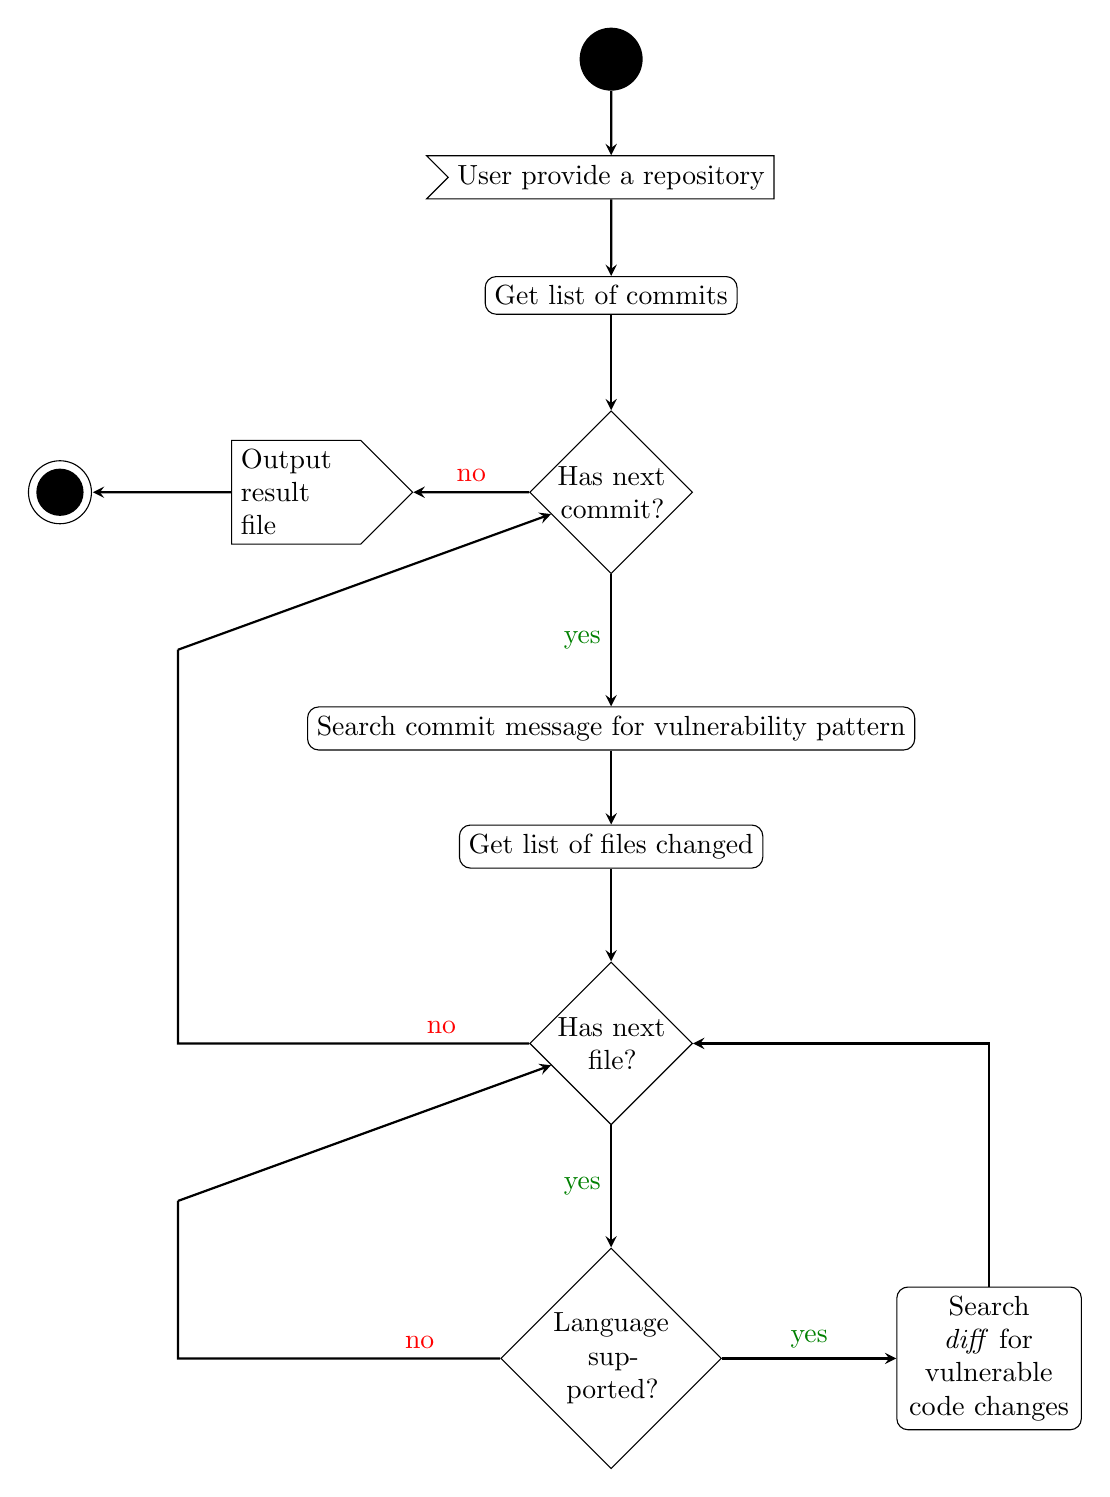
\begin{tikzpicture}
    [node distance=1.5cm,
    start/.style={circle, fill=black, minimum size=8mm},
    end/.style={path picture={\draw circle [radius=4mm]; \fill circle [radius=3mm];}},
    activity/.style={rectangle, draw, text centered, rounded corners},
    decision/.style={diamond, draw, text width=4em, text badly centered, inner sep=0pt,
    node distance=2.5cm},
    input/.style={signal, draw, signal from=west, signal to=nowhere},
    output/.style={signal, draw, signal to=east},
    arrow/.style={thick, ->, >=stealth}]
    \node [start] (start) {};
    \node [input, below of=start] (load_repo) {User provide a repository};
    \node [activity, below of=load_repo] (for_commit) {Get list of commits};
    \node [decision, below of=for_commit] (has_next_commit) {Has next commit?};
    \node [activity, below of=has_next_commit, node distance=3cm] (match_regex)
    {Search commit message for vulnerability pattern};
    \node [activity, below of=match_regex] (for_mods) {Get list of files changed};
    \node [decision, below of=for_mods] (has_next_file) {Has next file?};
    \node [decision, below of=has_next_file, text width=4.7em, node distance=4cm] (file_supported)
    {Language supported?};
    \node [activity, right of=file_supported, text width=6em, node distance=4.8cm] (search_diff)
    {Search \textit{diff} for vulnerable code changes};
    \node [output, left of=has_next_commit, text width=4em, node distance=4cm] (output) {Output
    result file};
    \node [end, minimum size=8.2mm, left of=output, node distance=3cm] (end) {};

    \draw [arrow] (start) -- (load_repo);
    \draw [arrow] (load_repo) -- (for_commit);
    \draw [arrow] (for_commit) -- (has_next_commit);
    \draw [arrow] (has_next_commit) -- node [anchor=east] {\textcolor{Green}{yes}} (match_regex);
    \draw [arrow] (has_next_commit) -- node [anchor=south] {\textcolor{Red}{no}} (output);
    \draw [arrow] (match_regex) -- (for_mods);
    \draw [arrow] (for_mods) -- (has_next_file);
    \draw [arrow] (has_next_file) -- node [anchor=east] {\textcolor{Green}{yes}} (file_supported);
    \draw [arrow] (has_next_file) -| node [very near start, anchor=south] {\textcolor{Red}{no}}
    (-5.5,-7.5) ++ (0,0) -- (has_next_commit);
    \draw [arrow] (file_supported) -- node [anchor=south] {\textcolor{Green}{yes}} (search_diff);
    \draw [arrow] (file_supported) -| node [very near start, anchor=south] {\textcolor{Red}{no}}
    (-5.5, -14.5) ++ (0,0) -- (has_next_file);
    \draw [arrow] (search_diff.north) |- (has_next_file.east);
    \draw [arrow] (output) -- (end);
  \end{tikzpicture}
  \caption{UML activity diagram of the repository mining tool}
  \label{figure:activity_diagram}
\end{figure}

The program flow of the repository mining tool is shown in
\hyperref[figure:activity_diagram]{\textbf{Figure \ref*{figure:activity_diagram}}}. It is an general
representation of the whole process. Hence, exhaustive details including exception handling,
function calls, and user inputs validation are not included.

\section{Commit Messages Matching} \label{sec:design_commit_matching}
As mentioned in \hyperref[sec:proposed_method]{\textbf{Section \ref*{sec:proposed_method}}}, there
is already a concept of how commit messages matching should be functioning. It can be defined as the
process of matching the commit message with the regular expression of each vulnerability pattern to
find vulnerability-fixing commit. It requires some prior knowledge of the vulnerability patterns to
define the regular expressions.

\subsection{Vulnerability Patterns and Regular Expressions}
The general idea of using regular expressions on commit messages is to construct the search queries
with multiple conditions. Searching with regular expressions enables the tool to get results with
one search, and avoid the usage of conditional statements to process the queries. Designing a
specific, complete, and correct regular expression is challenging. This research question has two
aspects to consider:
\begin{enumerate}
  \item \textbf{Completeness:} If the objective was to achieve high completeness, then the regular
  expression would be designed to cover a broad range of string patterns. This would match more
  commit messages with the regular expression, which might possibly find more positive results.
  Similarly, false positive rate and the effort required for manual evaluation would increase.
  \item \textbf{Correctness:} If the objective was to achieve high correctness, then the regular
  expression would be designed to be specific. This approach lowers the false positive rate, but
  increases the likelihood of generating false negatives.
\end{enumerate}

The ideal design is to achieve high completeness and high correctness, but this assumption is not
realistic. This is because the quality of commit messages is not reliable, as discussed in
\hyperref[subsec:commit_quality]{\textbf{Section \ref{subsec:commit_quality}}}. Achieving high
correctness (low false positive rate) is desirable, but the additional effort in the improvement
might not yield the corresponding improvements. Hence, the optimal approach would attempt to achieve
high completeness first, then perform refinement on the regular expressions based on the results.

\subsection{Expected Behaviour}
\begin{figure}[H]
  \centering
  \includegraphics[width=.85\textwidth]{images/keyword_search.png}
  \caption{An example of a search query \textbf{`\acrshort{cve}'} on GitHub.}
  \label{figure:keyword_search}
\end{figure}

Since regular expression is used instead of plain text search, the tool is aimed to perform at
least, or better than the GitHub search in \hyperref[figure:keyword_search]{\textbf{Figure
\ref*{figure:keyword_search}}}. However, the tool does not produce a \acrshort{gui} output
immediately after the search has completed, it stores the search results into a \acrshort{json} file
for manual evaluation.

\section{Vulnerable Code Searching} \label{sec:design_vuln_code_search}
Commit messages matching (\hyperref[sec:design_commit_matching]{\textbf{Section
\ref*{sec:design_commit_matching}}}) is not sufficient to prove the validity of the results. A
commit message does not always summarise the actual changes in the commit object. To correctly
identify a vulnerability-fixing commit, it is required to analyse the code changes.

\subsection{Code Searching Techniques}
There are several approaches to scan the source code for vulnerabilities, ranging from simple text
matching to complex data flow analysis. While The former is easier to build, and provides a quick
way to find some potential security problems in the source code; the latter provides more accurate
results, and it is able to detect complex vulnerabilities that involves nested control statements
and function calls \cite{castro_2006}.

To select an approach, this research question has to consider several factors:
\begin{enumerate} \label{subsec:code_searching}
  \item \textbf{Performance:} The amount of system resources and time required to complete one
  search of the chosen technique.
  \item \textbf{Complexity:} The difficulty of implementing such technique.
  \item \textbf{Feasibility:} The possibility measurement of producing a functional implemention of
  the chosen technique that satisfies the requirements.
  \item \textbf{Accuracy:} The measurement of the ability to correctly identify the vulnerable lines
  of code.
\end{enumerate}

\subsection{Chosen Technique}
After consideration of the factors listed in \hyperref[subsec:code_searching]{\textbf{Section
\ref*{subsec:code_searching}}}, it is chosen to implement a \textbf{static analysis technique}. It
has been widely used in many security analysis tools including SpotBugs \cite{spotbugs}, Flawfinder
\cite{flawfinder}, Bandit \cite{bandit}, and Progpilot \cite{progpilot}. As a result, it is required
to discuss the strengths and weaknesses of the chosen technique to obtain an abstract indication of
the expected results.

\subsection*{Strengths}
\begin{itemize}
  \item It scales accordingly to the code size. Unlike data flow analysis, it does not need to
  construct abstract syntax tree or control flow graph for its analysis process. Therefore, it is
  unlikely to encounter severe performance or memory issues.
  \item It is able to detect relatively simple vulnerabilities such as buffer overflows and SQL
  injections with high confidence. Although these vulnerabilities can sometimes be very  complex as
  well.
\end{itemize}

\subsection*{Weaknesses}
\begin{itemize}
  \item It is unable to detect many security vulnerabilities automatically and accurately. These
  security vulnerabilities usually require sophisticated analysis method to detect.
  \item It is expected to generate numberous false postiive results.
  \item It is difficult to prove the validity of the results. Since the analysis does not involve
  any data flow analysis, the reported results do not contain any detailed information such as
  variables value, and the steps to exploit the vulnerabilities.
\end{itemize}

\subsection{Severity and Confidence Level}
To mitigate the weaknesses, a severity and confidence level can be assigned to each vulnerability
identified. They give the user an indication about the seriousness of a vulnerability, and the
likelihood for the vulnerability to be correctly identified. With these parameters, the user can now
choose to filter the results with severity or confidence higher than a certain level. This would
lower the effort and time required for manual evaluation.

\section{Level of Detail in Result File} \label{sec:lod_result}
Every Git commit object contains a lot of metadata \cite{chacon_2014}. Storing all metadata of each
commit found will consume a substantial amount of storage space, as well as increasing the reading
time of the result file. Hence, only relevant information that will be used in statistical
evaluation are included, which are listed below:
\begin{enumerate}
  \item The commit message (optional)
  \item The date of the commit
  \item The matching groups of regular expression
  (\hyperref[sec:design_commit_matching]{\textbf{Section \ref*{sec:design_commit_matching}}})
  \item The vulnerability pattern of the matched regular expression
  (\hyperref[sec:design_vuln_code_search]{\textbf{Section \ref*{sec:design_vuln_code_search}}})
  \item The vulnerable code changes identified, with line number, code severity level, and
  confidence level. (\hyperref[sec:design_vuln_code_search]{\textbf{Section
  \ref*{sec:design_vuln_code_search}}})
\end{enumerate}

The commit message is just for the ease of user reference, which might be trivial as it does not
have positive usage for the analysis but storing it will increase the file size.

\section{Statistical Evaluation}
The final part of this project is to create a statistical analysis tool to analyse the result file
produced. The purpose to calculate these statistics is to study the relationship among
vulnerability-fixing commit, commit message, and lines changed. The proposed method is to load the
\acrshort{json} result file into a Python dictionary first, then calculate the statistics. Below is
a list of statistics to calculate in the statistical analysis tool:
\begin{enumerate}
  \item Total commits found
  \item A list of years that represents the number of commits found in each of the year
  \item A list of vulnerability types found by regular expressions match and vulnerable code search
  \item The number of commits found, calculated according to severity and confidence level
  \item The number of commits found that are \textbf{only} matched by regular expressions
  \item The number of commits found that \textbf{only} have vulnerable lines changed
  \item The number of commits found that have \textbf{both} regular expressions match and vulnerable
  lines changed
\end{enumerate}

\chapter{Implementation and Testing} \label{chap:implementation}
This chapter will discuss the implementation of the repository mining tool based on the
specifications described in previous chapters. It will also provide insights into the challenges
encountered during the implementation process.

\section{Project Environment and Structure}
\subsection{Hardware Requirements}
This project relies on strong processing power and high availability of memory (RAM). The speed of
the analysis process is determined by the processing power of the CPU. For large repositories, it is
recommended to allocate at least 4GB of RAM to the process, otherwise the process might encounter an
memory error and terminate.

\subsection{Software Requirements}
As concluded in \hyperref[subsec:prog_lang]{\textbf{Section \ref*{subsec:prog_lang}}}, the project
has been implemented in Python 3. There are several Python 3 versions available, and the project
used the latest stable version at the time of this project, which is Python 3.7.3. Specifically, the
source code is written with the new syntax and features introduced in the latest version, which
impies that the older versions of Python 3 are not able to run it before updating.

\subsection{Structure}
\hyperref[fig:directory_structure]{\textbf{Figure \ref*{fig:directory_structure}}} shows the
directory stucture of the project. It follows the design in
\hyperref[figure:class_diagram]{\textbf{Figure \ref*{figure:class_diagram}}}, where the file
\texttt{vulnerability.py} and \texttt{language.py} contain the class \texttt{Vulnerability} and
\texttt{Language} respectively. It is not necessary to create an individual file for each
programming language in the \texttt{languages} folder, but it is recommended in practice for better
maintainability and clarity of the project.

\begin{figure}[H]
  \centering
  \begin{forest}
    pic dir tree,
    where level=0{}{% folder icons by default; override using file for file icons
      directory,
    },
    [root
      [languages
        [\_\_init\_\_.py, file]
        [c.py, file]
        [java.py, file]
        [language.py, file]
        [python.py, file]
      ]
      [tests]
      [flawfinder.py, file]
      [shefmine.py, file]
      [shefstat.py, file]
      [vulnerability.py, file]
    ]
  \end{forest}
  \caption{Directory struture of the project} \label{fig:directory_structure}
\end{figure}

\section{Commit Messages Matching}
This section is an explanation of how the design defined in
\hyperref[sec:design_commit_matching]{\textbf{Section \ref*{sec:design_commit_matching}}} was
implemented. The implementation is split into three stages, and each subsection below represent one
of the stage.

\subsection{Vulnerabilities}
The vulnerabilities represent the type of vulnerability-fixing or vulnerability-inducing commit to
find. Each vulnerability is an instance of the class \texttt{Vulnerability}, and has a regular
expression pattern that indicates the possible string format of the commit messages. The
vulnerabilities below are implemented into the tool:

\begin{multicols} {2}
  \raggedright
  \begin{itemize}
    \item Broken Access Control
    \item Broken Authentication and Session Management
    \item Buffer Overflow
    \item Bug Tracker Issue
    \item Context Leaks
    \item Cross-Site Request Forgery
    \item Cross-Site Scripting
    \item Distributed Denial-of-Service / Denial-of-Service
    \item Encryption Issues
    \item Hard Coded
    \item Injection
    \item Insufficient Attack Protection
    \item Memory Leaks
    \item Miscellaneous
    \item Null Pointers
    \item Overflow
    \item Resource Leaks
    \item Path / Directory Traversal
    \item SHA-1 Collision
    \item Security Misconfiguration
    \item Sensitive Data Exposure
    \item Using Components with Known Vulnerabilities
    \item Underprotected APIs
  \end{itemize}
\end{multicols}

A new vulnerability can be created by passing two arguments to the \texttt{Vulnerability} class: the
name of the new vulnerability, and the regular expression pattern that describes the commit message
pattern, as demonstrated in \hyperref[code:create_vuln]{\textbf{Listing \ref*{code:create_vuln}}}.
\begin{lstlisting}[basicstyle=\ttfamily, label=code:create_vuln,
  caption=Creating a new instance of \texttt{Vulnerability}.]
Vulnerability(
  'Distributed Denial-of-Service / Denial-of-Service',
  '(dos|((distributed)? denial.*of.*service)|ddos|deadlocks?)')
\end{lstlisting}

\subsection{Writing the Regular Expressions}
Having defined the list of vulnerabilities to support, the next step is to write the regular
expression for each vulnerability. This is the most challenging part in commit message matching as
there are no specific definitions for the commit message format. Achieving \textbf{completeness} and
\textbf{correctness} is infeasible, it is impracticable to construct a regular expression that will
cover all the possible cases of a commit message.

The best mitigating approach is to assume that the commit messages of the same vulnerability type
would be having a similar format, or sharing some parts of a string. This could be accomplish with
the capturing group and wildcard character of regular expression. The graphical representation of
the regular expression \texttt{(fix|rem|patch|found|prevent).* mem.* leak|mem.* leak
(fix|removed?|patch|found|prevent)} is shown in \hyperref[figure:regex_groups]{\textbf{Figure
\ref*{figure:regex_groups}}}.

In real-world repositories, the regular expressions have a high possibility of matching a false
positive result. As discussed in \hyperref[subsec:commit_quality]{\textbf{Section
\ref*{figure:quality_commit_msg}}}, the quality of commit message is not reliable. This factor has
been considered into the final evaluation of the results.

\begin{figure}[H]
  \centering
  \includegraphics[width=.85\textwidth]{images/regex_groups.png}
  \caption{An example of using capturing groups and alternation in regular expression.}
  \label{figure:regex_groups}
\end{figure}

\subsection{Searching for the Matches}
The implementation for the search algorithm is not difficult since all regular expression operations
are already provided in the Python's \texttt{re} \cite{python_re} library. It is only required to
ensure that the operations will return the expected results for a given regular expression.

The algorithm is a single conditional statement. Given a commit message and a regular expression
pattern, if the commit message matches the regular expression pattern, then include the commit into
the result. As shown in \hyperref[code:commit_matching]{\textbf{Listing
\ref*{code:commit_matching}}}, the vulnerability name and matched string are saved into the result
file, which satisfied the requirements in \hyperref[sec:lod_result]{\textbf{Section
\ref*{sec:lod_result}}}.

\begin{lstlisting}[basicstyle=\ttfamily, label=code:commit_matching,
  caption=A partial snippet of the result file of CPython \cite{cpython_repo} repository.]
"de072100775cc29e6cd93a75466cecbd1086f258": {
  ...
  "vulnerabilities": [
    {
      "name": "Buffer Overflow",
      "match": "Fixed buffer overflow"
    }
  ],
  ...
},
"9790a2706573359e02fcfc5f18f9907467f4ec49": {
  ...
  "vulnerabilities": [
    {
      "name": "Sensitive Data Exposure",
      "match": "Fix for #1303614 and #1174712:\n- __dict__ des"
    }
  ],
  ...
}
\end{lstlisting}

The first commit in \hyperref[code:commit_matching]{\textbf{Listing \ref*{code:commit_matching}}} is
a successful example of the search, but the second commit is less specific and might require a
manual evaluation. In the second commit, the string `\texttt{for \#1303614 and
\#1174712:\textbackslash n- \_\_dict\_\_}' is a wildcard match. Although it is identified that the
second commit is a fix for some issues, the actual vulnerability fix might not a \texttt{Sensitive
Data Exposure} type.

\section{Vulnerable Code Searching} \label{sec:imp_vuln_code_search}
After commit message matching, the next step is to analyse the code changes in the commits. This
section will discuss the technique used to extract the information from the Git commit object, and
the use of the extracted information to find potential vulnerabilities in Git commit.

\subsection{Types of the Code Changes}
All code changes are recorded in the commit, and these changes can be categorised into added,
deleted, and unchanged.
\begin{itemize}
  \item \textbf{Added:} If an added line is reported as vulnerable, then the commit is identified as
  a vulnerability-inducing commit.
  \item \textbf{Deleted:} If an deleted line is reported as vulnerable, then the commit is
  identified as vulnerability-fixing commit.
  \item \textbf{Unchanged:} If an unchanged line in a changed file is detected as vulnerable, then
  it is possible for the repository to contain vulnerabilities that are not yet known.
\end{itemize}

It is important to note that the objective of the repository mining tool is to find potential
vulnerabilities through the commit history. Therefore, if a vulnerability is introduced at the very
first commit, and the file that contains the vulnerability has never been modified after that, then
it would not be possible for the tool to find it.

\subsection{Flawfinder and Bandit Integration} \label{subsec:flawfinder_bandit}
The Flawfinder program is a standalone tool and consists of only one file, but Bandit has a more
complex structure and consists of many classes. They were both written in Python and support at
least Python 2.7 and Python 3. Both of them are imported into the main file as modules, and their
functions can be directly invoked. No compatibility issues were countered during the integration
process.

Both Flawfinder and Bandit take a list of source files or directories as input from the
command-line, thus it is not able to pass the source code in a string form directly into the
functions. In GitPython \cite{gitpython}, the Diff object of a commit stores the old and new source
code as binary streams. The integration steps are:
\begin{enumerate}
  \item Decode the binary streams into string.
  \item Write the decoded source code into a temporary file.
  \item Pass the temporary file into the relative Flawfinder or Bandit function.
  \item The results will be returned when the Flawfinder or Bandit has finished the analysis.
\end{enumerate}

\subsection{User-defined Programming Language}
Python is an \acrfull{oop} language, it can fulfil the design specifications of
\hyperref[sec:supported_prog_lang]{\textbf{Section \ref*{sec:supported_prog_lang}}}. To support an
extra programming language, an instance of the \texttt{Language} class must be created. The
`constructor' (the \texttt{\_\_init\_\_} method) takes three parameters, a rule set, a list of file
extensions, and an optional regular expression object for non-context lines.

The importance and impact of the three parameters on the analysis results are explained below:
\begin{enumerate}
  \item \textbf{Rule set:} This is related to the core research objectives of this project. The
  repository mining tool will scan the source code with each rule in the rule set and record the
  matching one. A well defined rule set could reduce the possibility of false positives. However,
  there is a still limit on the effectiveness of it as the tool is only performing pure regular
  expression search with these rules on the source code. An example of the structure of a rule set
  is shown in \hyperref[code:ruleset]{\textbf{Listing \ref*{code:ruleset}}}.
  \begin{lstlisting}[basicstyle=\ttfamily, label=code:ruleset,
    caption=An example snippet of the Java ruleset.]
  ruleset = {
    'createStatement\s*\(.*\)': {
        'severity': 'HIGH',
        'confidence': 'LOW'
    },
    ...
  }
  \end{lstlisting}
  \item \textbf{File extensions:} Some programming languages use multiple file extensions as their
  source code file. The purpose of this parameter is to prevent the tool from carrying the search on
  irrelevant files.
  \item \textbf{Regular expression object for non-context lines:} The purpose of this parameter is
  to improve the accuracy and performance of the tool. By excluding the non-context lines from the
  analysis process, the tool is able to perform faster, and it is less likely to obtain false
  positive results. If this parameter is not provided, then the tool will analyse every single line
  of the source code.
\end{enumerate}

A rule can either be a plain string or a regular expression pattern, the algorithm will take the
rule and perform a word boundary search (\verb|\b{rule}\b|). In contrast to Flawfinder and Bandit,
this algorithm does not need to parse the source code and tokenise them in advance. With these
justifications, it is predicted that the tool would not have better performance than Flawfinder or
Bandit (\hyperref[subsec:flawfinder_bandit]{\textbf{Section \ref*{subsec:flawfinder_bandit}}}).

\section{Configurable Options}
As specified in \hyperref[subsec:chosen_model]{\textbf{Section \ref*{subsec:chosen_model}}}, the
repository mining tool is implemented as an executable Python script. This indicates that the
analysis process is customisable with command-line arguments.

\begin{itemize}
  \item The branch to analyse.
  \item The commit range to analyse. This can be specified by providing two dates, two tags, or two
  commit hash.
  \item The minimum severity level.
  \item The minimum confidence level.
\end{itemize}

\section{Exceptions and Errors}
An unhandled exception will cause the program to terminate. Exception occurs whenever syntactically
correct Python code results in an unhandled error. Below is a list of errors encountered during the
implementation and testing. The list does not include the errors that are already handled by
Flawfinder and Bandit.
\begin{itemize}
  \item \textbf{Decode error:} Not all binary streams are encoded in the same encoding. This error
  will occur when it is unable to decode the binary streams due to the encodings used is not
  supported by standard Python codecs.
  \item \textbf{Memory and storage error:} This error will occur when the tool is trying to output a
  very large result file but the memory and storage space allocated is not enough.
\end{itemize}

\subsection{Special Case}
There are cases where the analysis progress is completely frozen. For example, the commit
\href{https://github.com/apache/camel/commit/b9a311}{\texttt{b9a311}} has 17925 files changed, which
will cause the progress to be stucked for a long time. Therefore, the tool is programmed to skip a
commit if it has more than 100 files changed.

\section{Testing}
The system was tested both automatically and manually to ensure that each feature has functioned
correctly. Automatic testing covered the test cases written using the Python's unit testing library
\cite{unittest}. Manual testing mostly covered some edge cases and tried to reproduce some rare
errors to ensure that they will be handled by the system.

\subsection{System Environment}
\begin{longtable}{|p{5.6cm}|p{5.6cm}|>{\columncolor[HTML]{B7E1CD}}c|}
  \hline \endfirsthead
  \rowcolor[HTML]{D8D8D8}
  \multicolumn{1}{|c|}{Test Case} & \multicolumn{1}{|c|}{Expected Result} & Status \\ \hline
  Windows 10, Python 3.6 and above & The program runs & Pass \\ \hline
  Windows 10, Python 3.5 and below & Syntax error, program does not run & Pass \\ \hline
  Linux, Python 3.6 and above & The program runs & Pass \\ \hline
  Linux, Python 3.5 and below & Syntax error, program does not run & Pass \\ \hline
  macOS, Python 3.6 and above & Syntax error, program does not run & Pass \\ \hline
  macOS, Python 3.5 and below & Syntax error, program does not run & Pass \\ \hline
  \caption{Test cases of system environment.}
\end{longtable}

\subsection{Program Initialisation}
\begin{longtable}{|p{5.6cm}|p{5.6cm}|>{\columncolor[HTML]{B7E1CD}}c|}
  \hline \endfirsthead
  \rowcolor[HTML]{D8D8D8}
  \multicolumn{1}{|c|}{Test Case} & \multicolumn{1}{|c|}{Expected Result} & Status \\ \hline
  Providing an invalid path & Exception is handled and error message is printed & Pass \\ \hline
  Providing an invalid Git repository & Exception is handled and error message is printed & Pass \\
  \hline
  Specifying an invalid branch & Exception is handled and error message is printed & Pass \\ \hline
  Specifying an invalid commit hash & Exception is handled and error message is printed & Pass \\
  \hline
  Specifying an invalid commit range & Exception is handled and error message is printed & Pass \\
  \hline
  Providing valid options & Program starts to analyse & Pass \\ \hline
  \caption{Test cases of program initialisation.}
\end{longtable}

\subsection{Repository and Commit Properties}
\begin{longtable}{|p{5.6cm}|p{5.6cm}|>{\columncolor[HTML]{B7E1CD}}c|}
  \hline \endfirsthead
  \rowcolor[HTML]{D8D8D8}
  \multicolumn{1}{|c|}{Test Case} & \multicolumn{1}{|c|}{Expected Result} & Status \\ \hline
  Providing an empty Git repository & Analysis started but no result file output & Pass \\ \hline
  Analysing an empty commit & The commit is skipped & Pass \\ \hline
  Analysing a commit with binary files changed only & Binary files are excluded from analysis & Pass
  \\ \hline
  Analysing a commit with more than 100 files changed & The commit is skipped & Pass \\ \hline
  Decoding a file changed that has invalid characters & The characters are ignored, and analysis
  continues to run & Pass \\ \hline
  Decoding a file changed of non-supported encoding & The file is skipped & Pass \\ \hline
  \caption{Test cases of repository and commit properties.}
\end{longtable}

\subsection{Commit Message Matching}
\begin{longtable}{|p{5.6cm}|p{5.6cm}|>{\columncolor[HTML]{B7E1CD}}c|}
  \hline \endfirsthead
  \rowcolor[HTML]{D8D8D8}
  \multicolumn{1}{|c|}{Test Case} & \multicolumn{1}{|c|}{Expected Result} & Status \\ \hline
  Given a non-matching string and a regular expression & The search operation returned \texttt{None}
  & Pass \\ \hline
  Given a matching string and a regular expression & The search operation returned the correct
  matched groups & Pass \\ \hline
  \caption{Test cases of commit message matching.}
\end{longtable}

\subsection{Vulnerable Code Searching}
\begin{longtable}{|p{5.6cm}|p{5.6cm}|>{\columncolor[HTML]{B7E1CD}}c|}
  \hline \endfirsthead
  \rowcolor[HTML]{D8D8D8}
  \multicolumn{1}{|c|}{Test Case} & \multicolumn{1}{|c|}{Expected Result} & Status \\ \hline
  File extension is not supported & The file is skipped & Pass \\ \hline
  File is empty & No issues returned & Pass \\ \hline
  Analysing a commit that has vulnerable code added  & Vulnerabilities is saved into the
  `added' list & Pass \\ \hline
  Analysing a commit that has vulnerable code deleted & Vulnerabilities is saved into the `deleted'
  list & Pass \\ \hline
  Analysing a commit that has vulnerable code unchanged & Vulnerabilities is saved into the
  `unchanged' list & Pass \\ \hline
  \hline
  \caption{Test cases of vulnerable code searching.}
\end{longtable}

\subsection{Performance Testing}
\begin{itemize}
  \item \textbf{Control variables:} The hardware specifications
  \item \textbf{Independent variables:} The number of commits to analyse, the size of a commit
  (number of files changed, number of code changes)
  \item \textbf{Dependent variables:} The time taken to complete the analysis
\end{itemize}

\begin{figure}[H]
  \centering
  \begin{tikzpicture}
    \pgfplotstableread[col sep=comma]{repos_time.dat}\datatable
    \begin{axis}[
      width=\textwidth, height=6cm,
      title={\textbf{Time against Total Number of Commits}},
      title style={align=center},
      enlarge x limits=0.02,
      xlabel near ticks, xlabel=Total Number of Commits,
      table/col sep=comma,
      date coordinates in=y,
      yticklabel=\Hour,
      ylabel near ticks, ylabel=Time (hours),
      legend pos=north west
    ]
    \addplot [scatter, only marks, point meta=explicit symbolic, scatter/classes={
        a={mark=x,blue},
        b={mark=triangle*,red},
        c={mark=o,draw=black}% <-- don’t add comma
      },] table[meta=label] {\datatable};
    \legend{C/ C++,Java,Python}
    \end{axis}
  \end{tikzpicture}
  \caption{Number of potentially vulnerable commits found since 1990 in all repositories analysed.}
  \label{figure:perf_result}
\end{figure}

According to \hyperref[figure:perf_result]{\textbf{Figure \ref*{figure:perf_result}}}, it has been
shown that there is a positive correlation between the time taken and the total number of commits.
The details of the results are recordeed in \hyperref[table:perf_result]{\textbf{Table
\ref*{table:perf_result}}}.

Overall, the performance of the repository mining tool is considered fast after taking into account
that all files changed of the whole commit history are analysed in the testing. In a practical
scenario, the users might only be interested in the commits that newer than a specific date or tag.
If these options are specified, then the time taken would decrease as there are less commits to
analyse.

\chapter{Results and Discussion}
This chapter

\section{Results Overview}
Repositories are not randomly selected. Selected based on actual software usage of large software
vendor.

\begin{figure}[H]
  \centering
  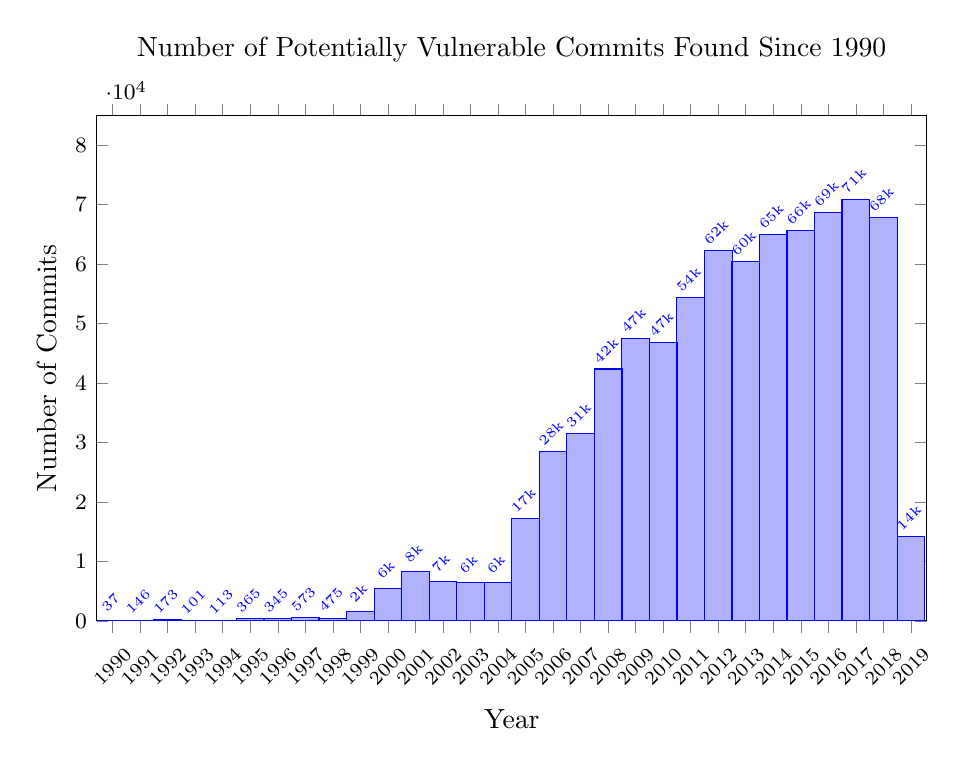
\begin{tikzpicture}
    \begin{axis}[
      width=\textwidth, height=8cm,
      title style={align=center, yshift=1em},
      title={Number of Potentially Vulnerable Commits Found Since 1990},
      xtick=data,
      x tick label style={/pgf/number format/1000 sep=, rotate=45, font=\scriptsize},
      xlabel near ticks, xlabel=Year,
      enlarge x limits=0.02,
      restrict x to domain=1970:2019,
      ylabel near ticks, ylabel=Number of Commits,
      ybar, ymin=0, ymax=85000,
      nodes near coords={
        \pgfkeys{/pgf/fpu=true, /pgf/fpu/output format=fixed}
        \pgfmathparse{\thenumber > 1000 ? \thenumber/1000 : \thenumber}
        \pgfmathprintnumber[precision=0]{\pgfmathresult}%
        \pgfmathparse{\thenumber > 1000 ? 1 : 0}%
        \pgfkeys{/pgf/fpu=false}%
        \pgfmathparse{\pgfmathresult > 0 ? "k" : ""}%
        \pgfmathresult
        },
      nodes near coords style={rotate=45, xshift=3pt, font=\tiny},
      visualization depends on=y \as \thenumber,
    ]
    \addplot coordinates {(1990, 37) (1991, 146) (1992, 173) (1993, 101) (1994, 113) (1995, 365)
    (1996, 345) (1997, 573) (1998, 475) (1999, 1591) (2000, 5512) (2001, 8294) (2002, 6652) (2003,
    6461) (2004, 6468) (2005, 17198) (2006, 28484) (2007, 31482) (2008, 42376) (2009, 47475) (2010,
    46850) (2011, 54332) (2012, 62334) (2013, 60464) (2014, 64928) (2015, 65717) (2016, 68757)
    (2017, 70924) (2018, 67828) (2019, 14270)};
    \end{axis}
  \end{tikzpicture}
  \caption{Number of potentially vulnerable commits found since 1990 in all repositories analysed.}
\end{figure}

\begin{table}[H]
  \centering
  \begin{tabular}{|l|l|l|}
    \hline
    \rowcolor[HTML]{D8D8D8}
    \multicolumn{1}{|c|}{Vulnerabilities} & \multicolumn{1}{|c|}{Total} &
    \multicolumn{1}{|c|}{Percentage} \\ \hline
    Broken Access Control & 190 & 0.13\% \\
    Broken Authentication and Session Management & 978 & 0.67\% \\
    Buffer Overflow & 1,365 & 0.94\% \\
    Bug Tracker Issue & 34,799 & 23.90\% \\
    Context Leaks & 17 & 0.01\% \\
    Cross-Site Request Forgery & 204 & 0.14\% \\
    Cross-Site Scripting & 310 & 0.21\% \\
    Distributed Denial-of-Service / Denial-of-Service & 7,340 & 5.04\% \\
    Encryption Issues & 24,291 & 16.68\% \\
    Hard Coded & 1,766 & 1.21\% \\
    Injection & 1,772 & 1.22\% \\
    Insufficient Attack Protection & 191 & 0.13\% \\
    Memory Leaks & 5,819 & 4.00\% \\
    Miscellaneous & 14,409 & 9.89\% \\
    Null Pointers & 7,803 & 5.36\% \\
    Overflow & 4,929 & 3.38\% \\
    Resource Leaks & 98 & 0.07\% \\
    Path / Directory Traversal & 177 & 0.12\% \\
    SHA-1 Collision & 1 & 0.00\% \\
    Security Misconfiguration & 10,457 & 7.18\% \\
    Sensitive Data Exposure & 22,657 & 15.56\% \\
    Using Components with Known Vulnerabilities & 186 & 0.13\% \\
    Underprotected APIs & 5,862 & 4.03\% \\ \hline \hline
    \textbf{Total} & \textbf{145,621} & \textbf{100.00\%} \\ \hline
  \end{tabular}
  \caption{Vulnerabilities matched by the regular expressions in all repositories analysed.}
\end{table}

\section{Case Study}

\section{Problems}
weakness of flawfinder:
memcpy() changes to memcpy () will be detected as well

In real-world repositories, there are many cases that will cause the

httpd repo
---------
\begin{itemize}
  \item \href{https://github.com/apache/httpd/commit/89fd8d}{\texttt{89fd8d}}: only comment changes
  \item \href{https://github.com/apache/httpd/commit/cd2b7a}{\texttt{cd2b7a}}: CVE in message,
  comment and code changes
\end{itemize}

CVE-2019-0211
Vulneable code searching is unable to detect very specific code
% https://github.com/apache/httpd/commit/a41bac
% https://httpd.apache.org/security/vulnerabilities_24.html
% https://cfreal.github.io/carpe-diem-cve-2019-0211-apache-local-root.html

Linux repo
\begin{itemize}
  \item \href{https://github.com/torvalds/linux/commit/224426f}{\texttt{224426f}}: date is year
  1970, parent is year 2007
  \item \href{https://github.com/torvalds/linux/commit/09f2724}{\texttt{09f2724}}: date is year
  2030, parent is year 2008
  \item \href{https://github.com/torvalds/linux/commit/12ca45f}{\texttt{12ca45f}}: date is year
  2030, parent is year 2008
\end{itemize}

\section{Evaluation}

\subsection{Verification and Validation}
After the implementation and testing has finished,

\section{Goals Achieved}
Overall, the repository mining tool has achieved the implementation objects and satisfied the
software requirements in \hyperref[sec:software_req]{\textbf{Section \ref*{sec:software_req}}}.

\section{Further Work}
pyhton multiprocessing

\chapter{Conclusion}

\printglossary[type=\acronymtype]
\printbibliography[heading=bibintoc]

\clearpage

\appendix
\chapter*{Appendices}
\markboth{APPENDICES}{}
\addcontentsline{toc}{section}{Appendices}
\setcounter{table}{0}
\renewcommand{\thetable}{A\arabic{table}}
\renewcommand{\thesubsection}{\Alph{subsection}}

\subsection{Performance Testing Results}
  \begin{longtable}{|l|l|l|}
    \hline \endfirsthead
    \multicolumn{1}{|c|}{Repository} & \multicolumn{1}{|c|}{Total commits} & \multicolumn{1}{|c|}
    {Time (hh:mm:ss)} \\ \hline
    \multicolumn{3}{|c|}{\cellcolor[HTML]{D8D8D8}C/C++} \\ \hline
    curl & 24,173 & 0:38:37 \\
    httpd & 31,399 & 1:16:21 \\
    icu & 30,642 & 9:03:57 \\
    ImageMagick & 15,503 & 1:12:41 \\
    libarchive & 5,461 & 0:13:15 \\
    libpng & 4,054 & 0:36:14 \\
    libtomcrypt & 1,906 & 0:04:01 \\
    libxml2 & 4,737 & 0:32:35 \\
    libxslt & 1,776 & 0:03:40 \\
    linux & 825,898 & 73:54:55 \\
    openssl & 23,714 & 0:54:28 \\
    v8 & 55,289 & 9:38:54 \\
    xalan-c & 4,323 & 0:07:38 \\
    xerces-c & 6,358 & 0:16:11 \\
    zlib & 419 & 0:01:29 \\ \hline
    \multicolumn{3}{|c|}{\cellcolor[HTML]{D8D8D8}Java} \\ \hline
    activemq & 10,158 & 0:32:46 \\
    axis2-java & 13,329 & 1:05:14 \\
    batik & 3,490 & 0:14:28 \\
    bc-java & 5,530 & 0:25:21 \\
    camel & 36,562 & 4:49:29 \\
    cocoon & 13,156 & 0:25:47 \\
    commons-fileupload & 950 & 0:00:38 \\
    cordova-android & 3,760 & 0:05:04 \\
    cxf & 14,879 & 1:24:13 \\
    flex-sdk & 33,707 & 1:22:20 \\
    geronimo & 13,137 & 0:27:42 \\
    httpcomponents-client & 2,993 & 0:09:33 \\
    jetty.project & 16,621 & 1:00:20 \\
    poi & 9,786 & 0:38:15 \\
    spring-framework & 18,415 & 0:56:35 \\
    spring-security & 7,616 & 0:12:14 \\
    struts & 5,649 & 0:09:16 \\
    tomcat & 20,723 & 0:54:59 \\
    wss4j & 2,543 & 0:12:30 \\
    xalan-j & 4,560 & 0:10:17 \\ \hline
    \multicolumn{3}{|c|}{\cellcolor[HTML]{D8D8D8}Python} \\ \hline
    ansible & 44,388 & 4:39:53 \\
    asn1crypto & 586 & 0:09:38 \\
    bcrypt & 165 & 0:00:25 \\
    botocore & 5,666 & 0:55:11 \\
    cpython & 103,752 & 17:01:44 \\
    cryptography & 7,619 & 1:09:44 \\
    django & 26,822 & 5:35:03 \\
    flask & 3,505 & 0:14:14 \\
    home-assistant & 18,675 & 1:56:53 \\
    paramiko & 3,231 & 0:13:29 \\
    photon & 3,433 & 0:04:22 \\
    pyopenssl & 1,999 & 0:33:27 \\
    python-certifi & 140 & 0:00:03 \\
    requests & 5,614 & 0:35:14 \\
    sqlmap & 8,671 & 0:42:55 \\
    tornado & 4,054 & 0:26:48 \\
    urllib3 & 3,190 & 0:20:28 \\ \hline \hline
    \textbf{Total (52 repos.)} & \textbf{1,514,726} & \textbf{148:31:28} \\ \hline
    \caption{The time taken to complete the analysis process of each repository.}
    \label{table:perf_result}
  \end{longtable}
\end{document}
